\RequirePackage[l2tabu, orthodox]{nag}
\RequirePackage{silence}
  \WarningFilter{biblatex}{Patching footnotes failed}
  \WarningFilter{hyperref}{Option `pdflang' has already been used}
  \WarningFilter{hyperref}{Option `pdfdisplaydoctitle' has already been used}
  % main.tex: Package biblatex Warning: Field 'prefixnumber' deprecated. Please use 'labelprefix' instead.
  \WarningFilter{biblatex}{Field 'prefixnumber' deprecated.}

\documentclass[sigconf,natbib=false]{acmart}

%drt24 hacks
% Letter paper
\setlength{\paperheight}{11in}
\setlength{\paperwidth}{8.5in}

%%% Handle input and output of accented/special characters and modern fonts
\usepackage[T1]{fontenc}
\usepackage[utf8]{inputenc}
\usepackage{lmodern}

%%% Better biblatex
\let\citename\relax
\usepackage[american]{babel}
\usepackage{csquotes}
\usepackage[style=ACM-Reference-Format,
  abbreviate=true, dateabbrev=true, isbn=true, doi=true, urldate=comp, url=true, eprint=false,
  maxnames=4, minnames=4, backref=false, backend=biber, language=american, sortcites=true,
  autocite=inline% , labelnumber=true
  ]{biblatex}
% \cite, \parencite, \footcite, \textcite, \autocite

\addbibresource{references/gecco2018.bib}
\renewcommand{\bibfont}{\Small}

%%% Include todo notes while writing draft (\listoftodos, \todo, \missingfigure)
\usepackage[color=white]{todonotes}

%%% Demo boxes
\usepackage{xcolor}
\newcommand\crule[3][black]{\textcolor{#1}{\rule{#2}{#3}}}

%%% Easier SI units
\usepackage[allowlitunits]{siunitx}

%%% Better looking tables
\usepackage{booktabs}
\renewcommand{\arraystretch}{1.2}
\usepackage{array}

%%% Better handling of links
\usepackage{url}

%%% Better math
\usepackage{amsmath}


%%% Colors for tracking changes
\newcommand{\red}[1]{\textcolor{red}{#1}}
\newcommand{\blue}[1]{\textcolor{blue}{#1}}

%%% Commands for easily changing formatting (e.g., italicize)
\newcommand{\etal}{et~al.}
\newcommand{\ie}{i.e.}
\newcommand{\eg}{e.g.}

\newcommand{\figref}[1]{Figure~\ref{#1}}
\newcommand{\tblref}[1]{Table~\ref{#1}}
\newcommand{\secref}[1]{Section~\ref{#1}}


% Copyright
\setcopyright{rightsretained}
\acmDOI{10.1145/nnnnnnn.nnnnnnn}
\acmISBN{978-x-xxxx-xxxx-x/YY/MM}
\acmConference[GECCO '18]{the Genetic and Evolutionary Computation Conference 2018}{July 15--19, 2018}{Kyoto, Japan}
\acmYear{2018}
\copyrightyear{2018}
\acmArticle{4}
\acmPrice{15.00}

% Removes citation information below abstract
\settopmatter{printacmref=false}


\begin{document}
\title{Comparing Finite State MacHines and Artificial Neural Networks for Controlling a UGV}
% \titlenote{Produces the permission block, and copyright information}
% \subtitle{Extended Abstract}
% \subtitlenote{The full version of the author's guide is available as  \texttt{acmart.pdf} document}


\author{Anthony J. Clark}
\affiliation{%
  \institution{Missouri State University}
  \city{Springfield}
  \state{Missouri}
  \country{USA}
}
\email{AnthonyClark@MissouriState.edu}

\author{Jared M. Moore}
\affiliation{%
  \institution{Grand Valley State University}
  \city{Grand Rapids?}
  \state{Michigan}
  \country{USA}
}
\email{jared@email.com}


% Maximum 200 words

\begin{abstract}

%%% Background
% This section should be the shortest part of the abstract and should very briefly outline the following information:
% - What is already known about the subject, related to the paper in question
% - What is not known about the subject and hence what the study intended to examine (or what the paper seeks to present)
Unmanned ground vehicles (UGVs) are well suited to tasks that are either too dangerous or too monotonous for people. For example, UGVs can traverse arduous terrain in search of disaster victims.
%
However, it is difficult to design these system so that they perform well in a variety of different environments.
%
%
%
%%% Methods
% The methods section is usually the second-longest section in the abstract. It should contain enough information to enable the reader to understand what was done, and how.
In this study, we evolve controllers and physical characteristics of a UGV with transformable wheels to improve its mobility in a simulated environment.
%
The UGV's mission is to visit a sequence of coordinates while automatically handling obstacles of varying sizes by extending wheel struts radially outward from the center of each wheel.
%
Evolved finite state machines (FSMs) and artificial neural networks (ANNs) are compared, and a set of controller design principles are gathered from analyzing these experiments.
%
%
%
% Results
% The results section should be the longest part of the abstract and should contain as much detail about the findings as the journal word count permits.
%
Results show comparable performance between FSM and ANN controllers, but the evolved strategies differ.
%
% The final controller is designed to take advantage of both approaches: (1) the control system is no longer a black-box and can be predictably understood (unlike the ANN), and (2) it takes advantage of the continuous nature of an ANN.
%
%
%
% Conclusion
% This section should contain the most important take-home message of the study, expressed in a few precisely worded sentences. Usually, the finding highlighted here relates to the primary outcome measure; however, other important or unexpected findings should also be mentioned. It is also customary, but not essential, for the authors to express an opinion about the theoretical or practical implications of the findings, or the importance of their findings for the field. Thus, the conclusions may contain three elements:
% - The primary take-home message
% - The additional findings of importance
% - The perspective
% UGVs are valuable in many domains, however, they must be designed to work in many different environments.
%
Furthermore, we show that a UGV's controller and physical characteristics can be effectively chosen by examining results from evolutionary optimization.

\end{abstract}




% Unmanned ground vehicles (UGVs) are well suited to tasks that are either too dangerous or too monotonous for people. For example, UGVs can traverse arduous terrain in search of disaster victims. However, it is difficult to design these system so that they perform well in a variety of different environments. In this study, we evolve controllers and physical characteristics of a UGV with transformable wheels to improve its mobility in a simulated environment. The UGV's mission is to visit a sequence of coordinates while automatically handling obstacles of varying sizes by extending wheel struts radially outward from the center of each wheel. Evolved finite state machines (FSMs) and artificial neural networks (ANNs) are compared, and a set of controller design principles are gathered from analyzing these experiments. Results show comparable performance between FSM and ANN controllers, but the evolved strategies differ. Furthermore, we show that a UGV's controller and physical characteristics can be effectively chosen by examining results from evolutionary optimization.


%
% The code below should be generated by the tool at
% http://dl.acm.org/ccs.cfm
% Please copy and paste the code instead of the example below.
%
\begin{CCSXML}
<ccs2012>
<concept>
<concept_id>10010520.10010553.10010554.10010556.10011814</concept_id>
<concept_desc>Computer systems organization~Evolutionary robotics</concept_desc>
<concept_significance>500</concept_significance>
</concept>
<concept>
<concept_id>10010147.10010178.10010213.10010204.10011814</concept_id>
<concept_desc>Computing methodologies~Evolutionary robotics</concept_desc>
<concept_significance>300</concept_significance>
</concept>
</ccs2012>
\end{CCSXML}

\ccsdesc[500]{Computer systems organization~Evolutionary robotics}
\ccsdesc[300]{Computing methodologies~Evolutionary robotics}

\keywords{evolutionary robotics, artificial neural network, finite state machine, adaptive, unmanned ground vehicle}

\maketitle

% TODO:
% - compare final results with novel environment (different way-points)
% - textit vs emph vs mathit


\section{Introduction}


% (1) Introductory paragraph: Very briefly: What is the problem and why is it relevant to the audience attending *THIS CONFERENCE*? Moreover, why is the problem hard, and what is your solution? You must be brief here. This forces you to boil down your contribution to its bare essence and communicate it directly.
Autonomous unmanned ground vehicles (UGV) provide an excellent solution to tasks that require searching or monitoring in environments deemed too remote or dangerous for humans.
%
Consider \emph{search and rescue}: after a natural disaster a UGV can be used by first responders to help locate victims in unstable and hazardous locations.
%
% Compared with an unmanned aerial vehicle (UAV), a
UGVs have long operating durations, can carry heavy payloads (\eg{}, sensors), and can search in narrow and covered places such as forests and caves.
%
% Ideally, a heterogeneous swarm of UAVs and UGVs would coordinate to gain the advantages of both search modes~\citep{Kruijff.SearchAndRescue.ICFSR.2014}.
%
% In this paper, however, we limit our investigation to UGVs.
% In particular, we show results for improving the mobility of Adabot, a UGV that includes wheel struts.


% (2) Background paragraph: Elaborate on why the problem is hard, critically examining prior work, trying to tease out one or two central shortcomings that your solution overcomes.
% One issue that arises during the design of a UGV is how to ensure that the system
Ensuring that a UGV can handle many different types of terrain is an ongoing challenge.
%
Researchers have invented several different methods for addressing the issue of mobility in varied terrain.
%
Specifically, robots have been designed with treaded wheels, tracks, legged-wheels (wheels are rimless, wheel spokes make contact with the ground), wheeled-legs (wheels are on the end of legs and the suspension is potentially actively actuated), and transformable wheels~\citep{Saranli.IntJrnRoboRes.RHex.2001,Quinn.IROS.Whegs.2002,Eich.SSRR.Stair-climb-SAR.2008,Haldane.ICRA.VelociRoACH.2013,Kenneally.IEEERobAutLetters.Legged-robots.2016}.
%
Although these systems provide an advantage over traditional wheeled robots, optimization is not performed in the vast majority of these studies.
%
% \blue{How could EA help?}


% (3) Transition paragraph: What keen insight did you apply to overcome the shortcomings of other approaches? Structure this paragraph like a syllogism: Whereas P and P => Q, infer Q.
The device in this study, the \emph{Adabot} (see \figref{fig:adabot}), includes transformable wheels that can smoothly be converted from a round wheel, to a wheel with tire \emph{studs}, to a legged-wheel.
%
Wheel transformations are performed by extending wheel struts radially outward from the center of the wheel (see \figref{fig:wheel-extender}).
 % (see \secref{sec:adabot} for details \ref{sec:adabot} \nameref{sec:adabot}).
%
Adabot has been optimized using an evolutionary algorithm such that its physical characteristics and its controller are better able to handle terrain that includes obstacles of varying sizes.
%
In previous work~\citep{Clark.2017.SSCI.Adabot}, a similar system was optimized to maximum forward velocity over uneven terrain.
%
The present study differs in two main ways: (1) here we evolve controllers for a more difficult task: \emph{way-point following}, and (2) we analyze results from evolving two controller types of feedback controllers (rather than feed-forward).



% (4) Details paragraph: What technical challenges did you have to overcome and what kinds of validation did you perform?
In this study, we evolve the robot's chassis dimensions, its wheel radius, the number of wheel struts,
% (described in \secref{sec:adabot}),
along with either a finite state machine (FSM) controller or an artificial neural network (ANN) controller.
%
The best evolved FSMs and ANNs are analyzed and compared.
%
For this initial work, to ensure that we are able to effectively analyze the ANN, the network only has three input nodes, zero hidden nodes, and three output nodes. The inputs are fully connected to the outputs.
%
The network is only slightly more complex than a Type 2 Braitenberg vehicle~\citep{Braitenberg.Vehicles.Book.1986}.
%
Conclusions drawn from our analysis are used to create a set of design principles for a new controller that takes advantage of both techniques.
%
In particular, it is attractive to design a controller that is not a black-box like an ANN but less rigidly defined than an FSM.
%
% \blue{hybrid controller}
%
%
% (5) Assessment paragraph: Assess your results and briefly state the broadly interesting conclusions that these results support. This may only take a couple of sentences. I usually then follow these sentences by an optional overview of the structure of the paper with interleaved section callouts.
% The results presented in this study demonstrate how a UGV can be optimized to improve robustness.
%
% Specifically, evolving Adabot has made it more robust in the presence of varied terrain.
%
% The techniques and concepts presented in this study can be applied to the optimization of any physical system.
%
Source code has been made available on GitHub\footnote{\url{https://github.com/anthonyjclark/adabot02-ann}}.

% \vspace{-0.1in}

\begin{figure}[!ht]
    \centering

    % \subfloat[]{\fbox{\crule[white]{0.4\columnwidth}{2cm}}}
    % \hfil
    % \subfloat[]{\fbox{\crule[white]{0.4\columnwidth}{2cm}}}

    \subfloat[3D Printed Prototype]{%
        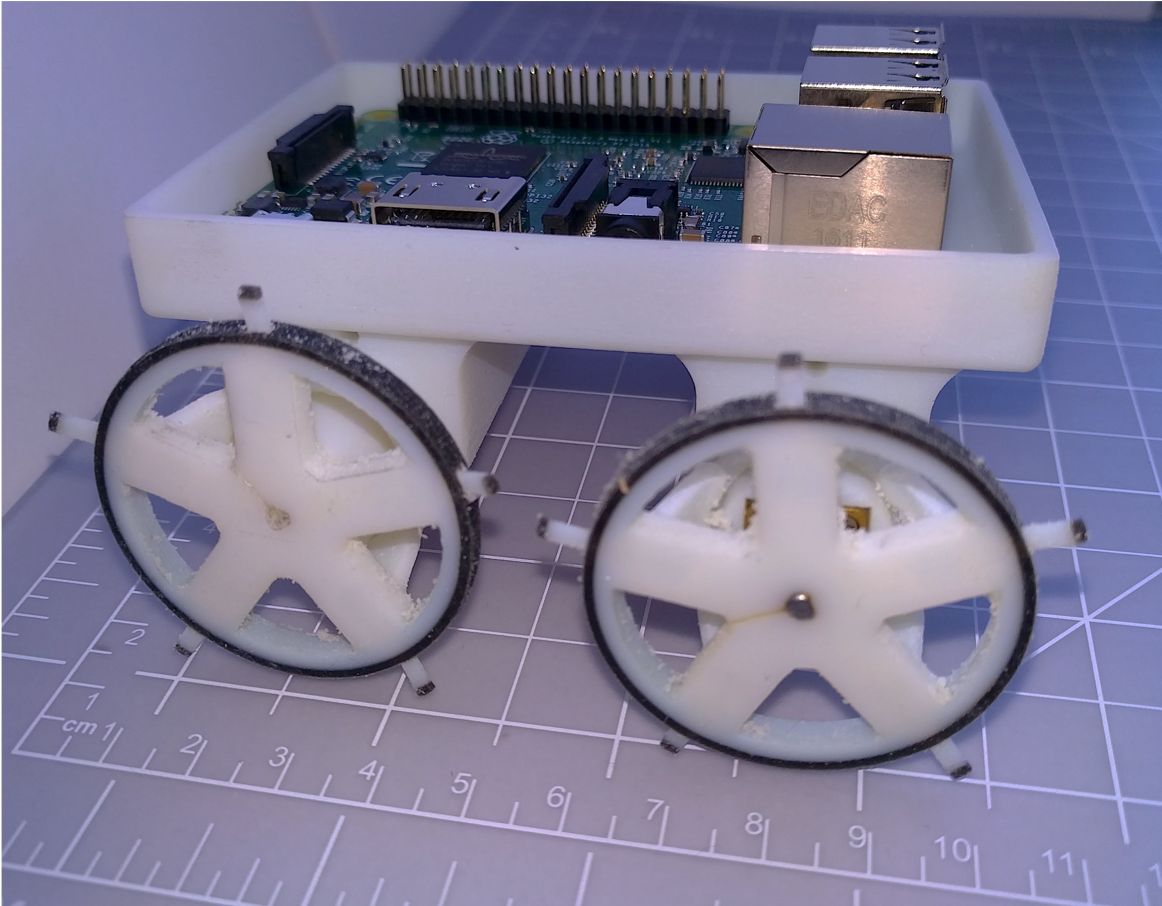
\includegraphics[width=0.2\textwidth,valign=c]{figures/1-introduction/perspective-image.jpg}%
    }\quad
    \subfloat[Simulated Device]{%
        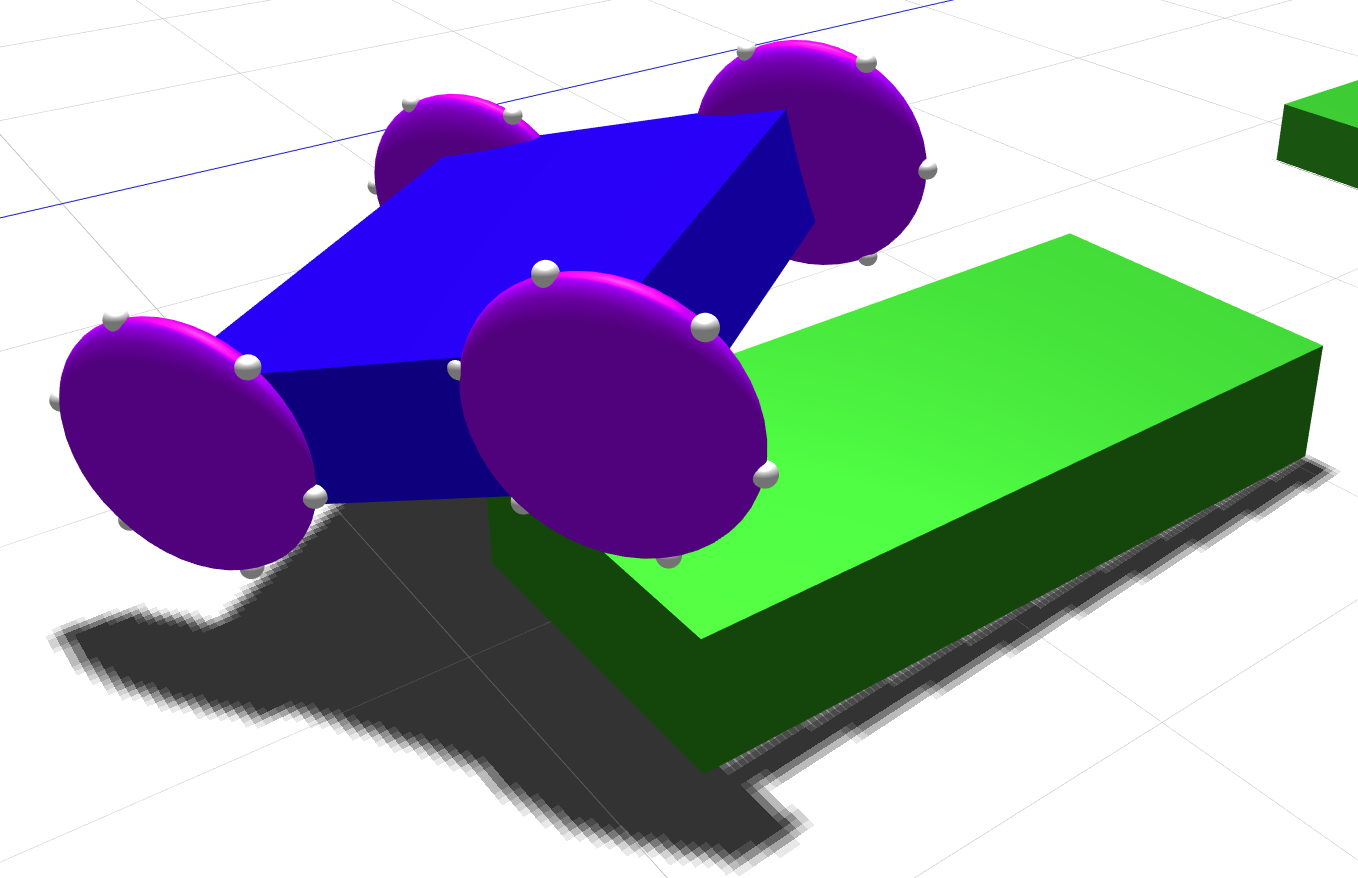
\includegraphics[width=0.2\textwidth,valign=c]{figures/1-introduction/simulation-climbing.png}%
        \vphantom{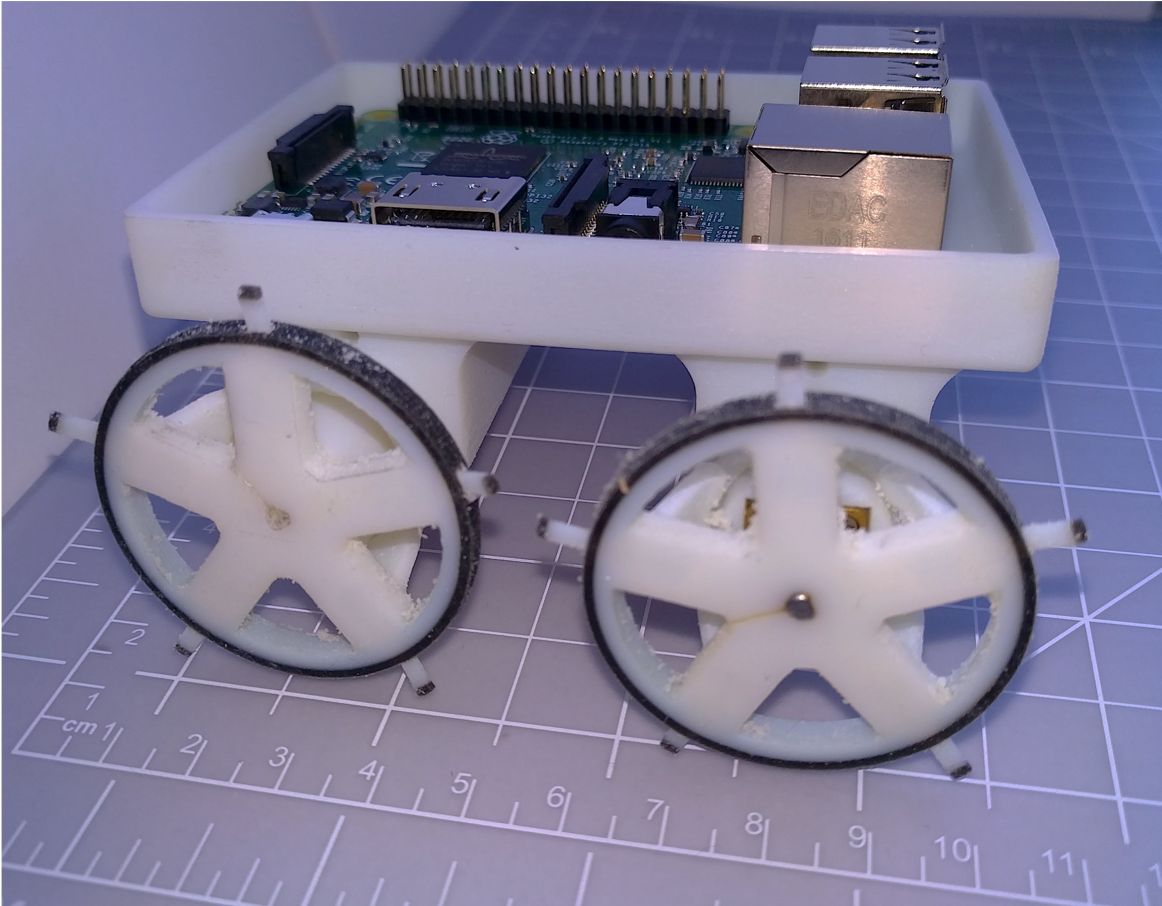
\includegraphics[width=0.2\textwidth,valign=c]{figures/1-introduction/perspective-image.jpg}}%
    }

    \vspace{-0.05in}

    \caption{Adabot, a UGV with transformable wheels.}
    \label{fig:adabot}

    \vspace{-0.15in}

\end{figure}

% \vspace{-0.1in}

% \input{sections/_2-background}
% \section{Adabot}
\label{sec:adabot}

In this section, we describe the prototype Adabot hardware, including the transformable wheel mechanism, along with the simulation environment utilized during evolutionary optimization.

% Hardware
% \subsection{Hardware}
% \paragraph{Hardware}
\vspace{0.1in}
\noindent
\textbf{Hardware}
%
The Adabot, pictured in \figref{fig:adabot}, is a prototype device that includes a Raspberry Pi 3 Model B (RPi) as its main control board.
%
The RPi was chosen for its ability to run the Robot Operating System (ROS)~\autocite{Quigley.ICRAOSS.ROS.2009}, which Adabot uses to manage its software systems.
%
The size of an RPi constrains the minimum dimensions of the Adabot's chassis. Specifically, the chassis must be at minimum 8~\si{cm} by 8~\si{cm}.
%
\tblref{tbl:params-physical} lists all configurable parameters for Adabot's physical characteristics, where
$\mathit{WheelBase}$ and $\mathit{TrackWidth}$ denote the distance between the front and rear axles and the lateral distance between wheels, respectively, and $\mathit{StrutCount}$ parameter indicates the number of struts per wheel.

\begin{table}[hb]
    \centering
    \caption{Adabot Physical Parameters}
    \label{tbl:params-physical}
    \begin{tabular}{@{}ll@{}}
        \toprule
        \textbf{Name} & \textbf{Range}\\
        \midrule
        $\mathit{WheelBase}$    & \numrange{8}{16}~\si{cm}\\
        $\mathit{TrackWidth}$    & \numrange{8}{16}~\si{cm}\\
        $\mathit{WheelRadius}$ & \numrange{2}{3}~\si{cm}\\
        $\mathit{StrutCount}$        & \numrange{0}{7}\\
        \bottomrule
    \end{tabular}
\end{table}



Each of the four wheels is driven by its own DC gear-motor with magnetic encoders.
%
Likewise, each wheel includes a set of struts that can be extended and retracted by a linear servo.
%
For sensing, Adabot includes three forward facing distance sensors and an IMU (3-axis gyroscope, 3-axis accelerometer, and 3-axis magnetometer).
%
Finally, it uses a 2.4 GHz wireless communication module and is powered by a 2200 mAh battery pack, which provides roughly two hours of operating time.


% Extension
% \subsection{Extender Mechanism}
% \paragraph{Extender Mechanism}
\vspace{0.1in}
\noindent
\textbf{Strut Extension}
%
\figref{fig:wheel-extender} depicts the strut extension process.
%
This mechanism enables the wheel to exhibit a range of characteristics.
%
With the struts fully retracted, the wheels operate conventionally; when extended a small amount the struts act as tire studs; and with the struts fully extended each wheel resembles a legged-wheel.
%
The radius of the wheel and the number of struts are both free parameters that can be evolved during optimization.
%
For the following discussion, the most important aspect of this mechanism is that the maximum extension of the struts is equal to 1~\si{cm} minus the wheel's radius ($\mathit{MAXEXT} = \mathit{WheelRadius} - 1~\si{cm}$).
%
For a more detailed discussion of Adabot's software and wheel extension mechanism, and an example of evolving Adabot with ROS and Gazebo (a simulation environment tightly coupled with ROS)~\parencite{Koenig.IROS.Gazebo.2004} see our preliminary study~\red{<citation removed to preserve anonymity>}.



\begin{figure}[!ht]
    \centering

    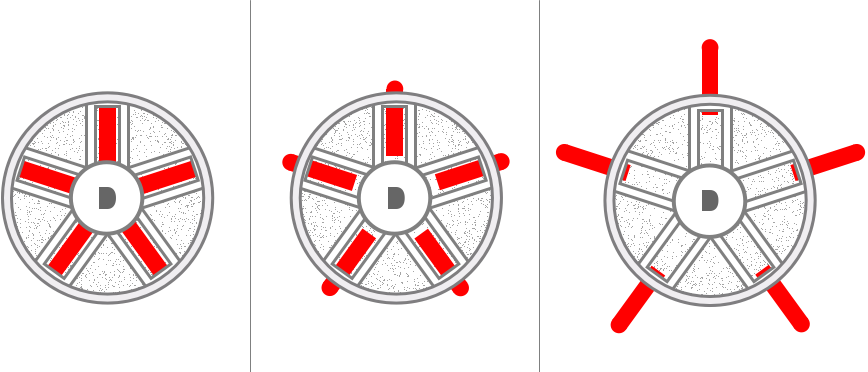
\includegraphics[width=\columnwidth]{figures/3-adabot/extension-mechanism.png}
    % \fbox{\crule[white]{\columnwidth}{2cm}}

    \vspace{-0.08in}

    \caption{An illustration of the Adabot's wheel extension mechanism, where the struts are fully retracted (left), partially extended (middle), and fully extended (right).}
    \label{fig:wheel-extender}

    \vspace{-0.15in}

\end{figure}

% Simulation
% \subsection{Simulation}
% \paragraph{Simulation}
\vspace{0.1in}
\noindent
\textbf{Simulation}
%
% As is the case for most ER studies, we use simulation during the optimization process.
%
An image of the simulation environment is shown in \figref{fig:simulation-environment}.
%
% To populate the environment with obstacles, we generate 40 boxes with random dimensions, positions, and densities.
The environment is populated by generating 40 boxes with random dimensions, positions, and densities.
%
If a newly generated box collides with another box it is removed from the simulation. We see on average 31 boxes in the environment.
%
Box heights are in the range \numrange{2}{5}~\si{cm}, which is high enough compared to the potential $\mathit{WheelRadius}$ values that most traditional wheeled robots will have difficulty climbing them~\autocite{Quinn.IROS.Whegs.2002}.
%
Moreover, rather than each box being in a fixed position, it is possible for the Adabot to push a box (depending on its size and density).


For this study, we are using the Dynamic Animation and Robotics Toolkit (DART)\footnote{https://dartsim.github.io/index.html}.
%
DART is specifically designed for robotics applications (unlike the Open Dynamics Engine\footnote{https://bitbucket.org/odedevs/ode}, which we've used in the past), and is comparable in speed (if not faster) than common alternatives~\autocite{Mouret.2017.SimER.Simulation}.
%
In this study, we do not simulate noise, and we assume that the robot has direct access to its global position and rotation. Essentially, we are mimicking a lab setup with an overhead camera that communicates directly with the robot.


\begin{figure}[!ht]
    \centering

    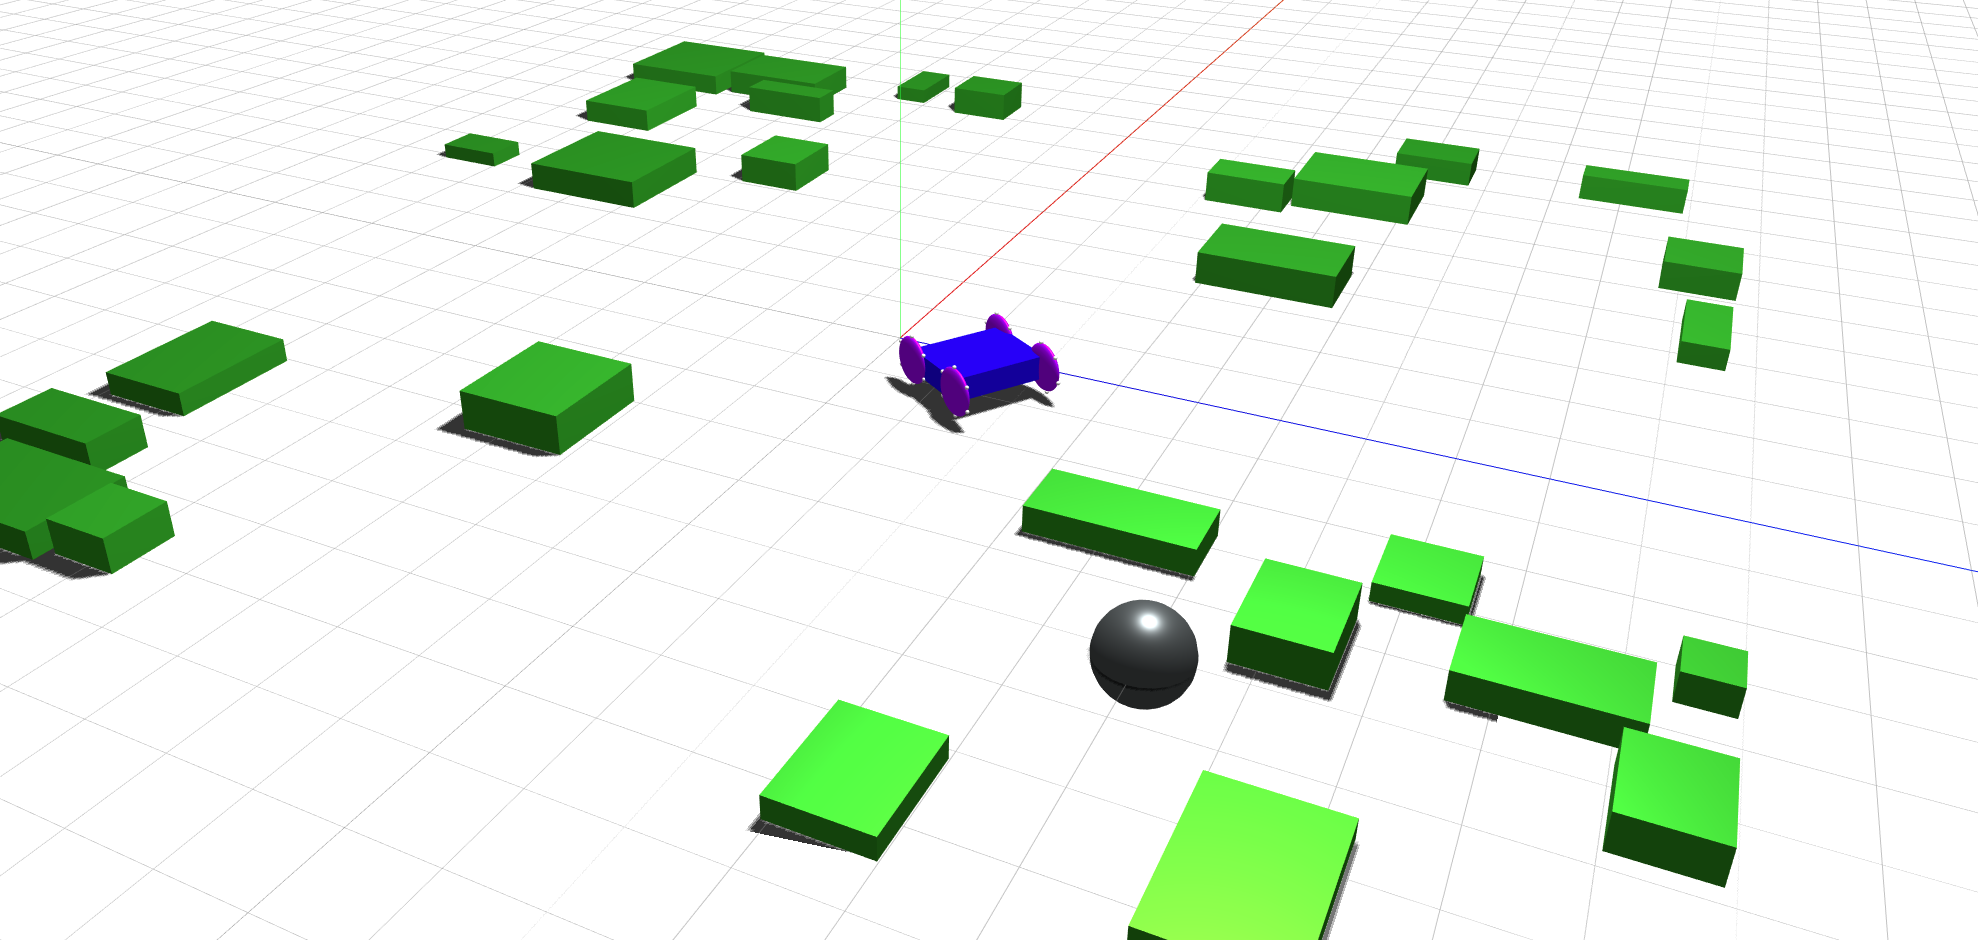
\includegraphics[width=0.8\columnwidth]{figures/3-adabot/environment.png}
    % \fbox{\crule[white]{\columnwidth}{2cm}}

    \vspace{-0.1in}

    \caption{An example environment including randomly generated obstacles. The current way-point is shown in dark gray, and the robot starts at the origin facing in the positive x-axis (away from the way-point, along the red axis line).}
    \label{fig:simulation-environment}

    \vspace{-0.2in}

\end{figure}

% Control Properties
% \subsection{Way-Point Navigation Control}
% \paragraph{Way-Point Navigation Control}
\vspace{0.1in}
\noindent
\textbf{Way-Point Navigation Control}
%
Adabot is a skid-steer style robot--it turns by rotating its left and right wheels at different rates. Although each wheel (and wheel strut set) can be controlled independently, in this study we only have three control outputs: (1) an angular rate for the left wheels, (2) and angular rate for the right wheels, and (3) a single extension amount for all four sets of struts.
%
For Adabot to aid during a search and rescue operation, it must be able to successfully \emph{cover} (completely search) its designated area.
%
A simplified version of this task, called \emph{way-point navigation}, is considered during evolutionary optimization.
%
For this task, a UGV must visit a set of way-points in sequence.
%
% Way-point navigation is the task that we consider during evolutionary optimization.
% We consider way-point navigation


\vspace{0.1in}
\noindent
\textbf{FSM Control}
A hand-designed FSM for this task is depicted in \figref{fig:fsm}(a).
%
This FSM includes two independent actions: (1) directing the robot towards the next way-point by controlling the left and right wheels, and (2) extending the struts when the robot is experiencing reduced mobility due to an obstacle.



The first action is handled by the three states shown in the top-half of the figure. Essentially, the robot remains in the \emph{Forward} state as long as the angle between the heading of the UGV and the direction to the target ($\alpha_{\mathit{target}}$) is within some threshold.
%
Once the threshold is surpassed, the FSM transitions to either the \emph{Left} or \emph{Right} state.
%
In the \emph{Left} and \emph{Right} states, the robot will rotate in place until $\alpha_{\mathit{target}}$ is less than another threshold, after which point the FSM transitions back to \emph{Forward}.
%
Threshold angles are shown in \figref{fig:fsm}(b).

\begin{figure*}[!ht]
    \centering

    % \includegraphics[width=0.6\columnwidth]{figures/4-simulation/state-machine.png}
    % \subfloat[]{\fbox{\crule[white]{0.4\columnwidth}{2cm}}}
    \subfloat[Direction Control]{%
        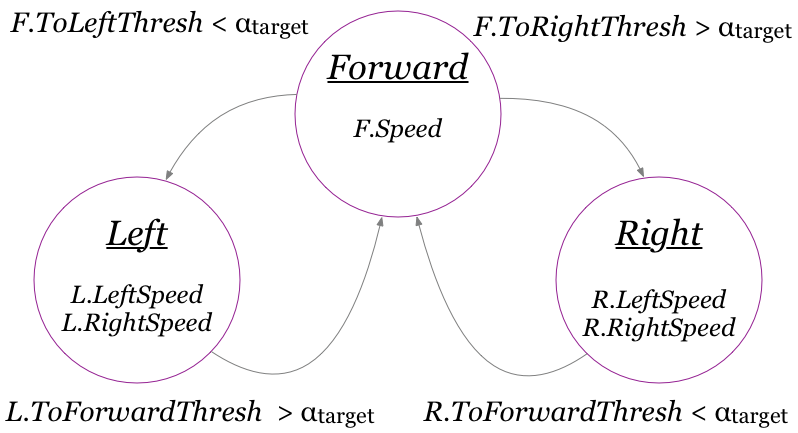
\includegraphics[width=0.3\textwidth,valign=c]{figures/3-adabot/FSM-direction.png}%
        \vphantom{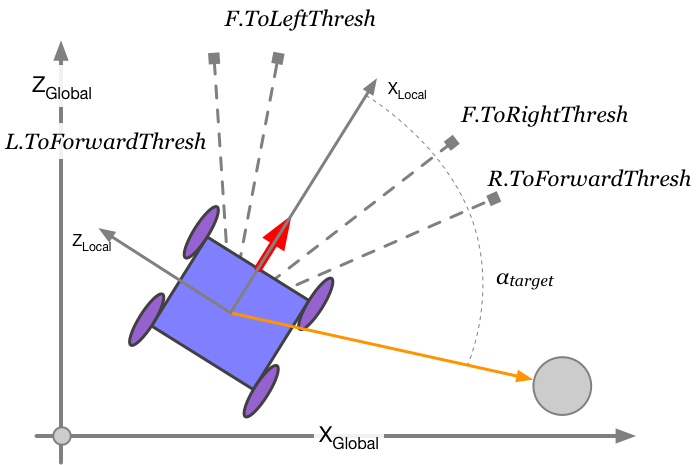
\includegraphics[width=0.3\textwidth,valign=c]{figures/3-adabot/scene.png}}%
    }
    \hfil
    \subfloat[Strut Extension Control]{%
        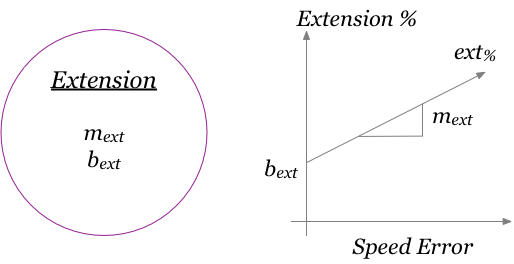
\includegraphics[width=0.2\textwidth,valign=c]{figures/3-adabot/FSM-strut.png}%
        \vphantom{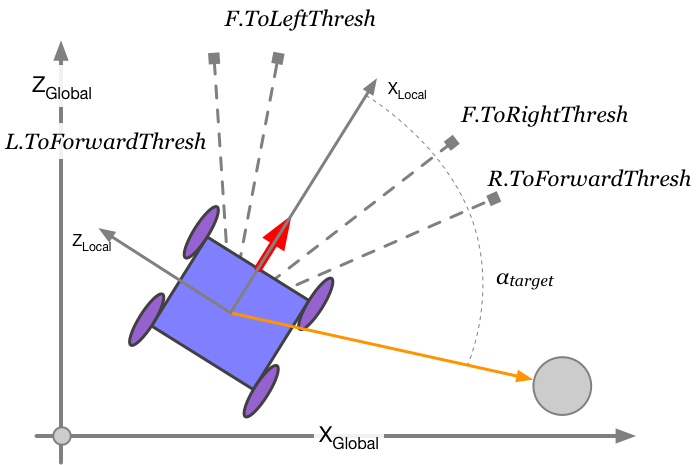
\includegraphics[width=0.3\textwidth,valign=c]{figures/3-adabot/scene.png}}%
    }
    \hfil
    \subfloat[Environment Diagram]{%
        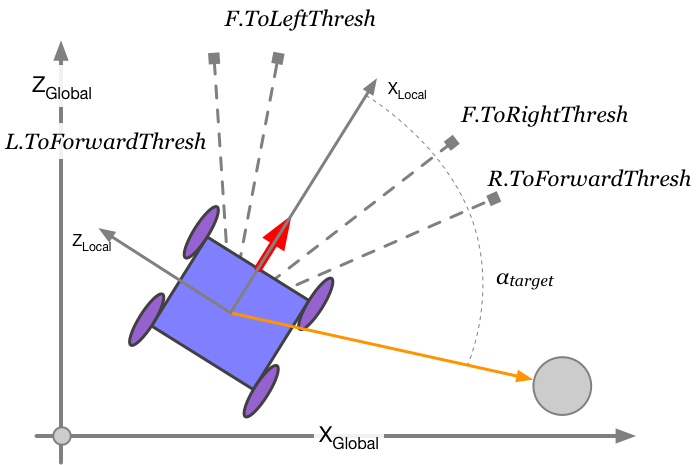
\includegraphics[width=0.3\textwidth,valign=c]{figures/3-adabot/scene.png}%
        \vphantom{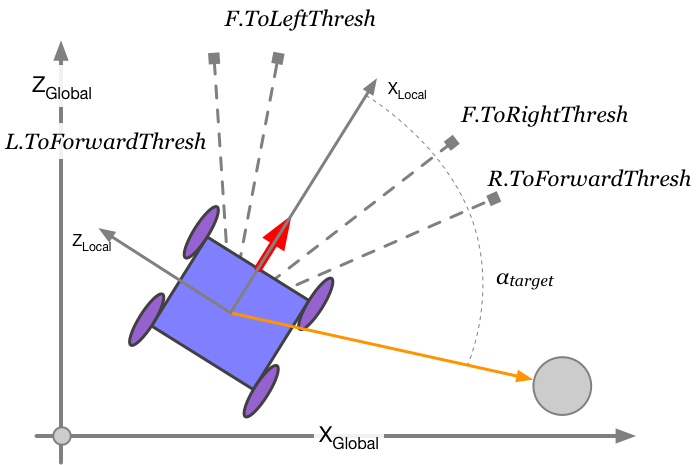
\includegraphics[width=0.3\textwidth,valign=c]{figures/3-adabot/scene.png}}%
    }

    \vspace{-0.08in}

    \caption{(a) The FSM controlling the direction of the robot, (b) the single state controlling wheel struts, and (b) a diagram depicting the angles used to trigger transitions between states.}
    \label{fig:fsm}

    \vspace{-0.1in}

\end{figure*}



The second action, handling the wheel struts, is accounted for by the state shown in the lower part of \figref{fig:fsm}(a).
%
This state calculates the expected linear ($v_{\mathit{UGV}}$) and angular ($\omega_{\mathit{UGV}}$) speed using a simple differential drive model:

\vspace{-0.08in}

\begin{align}
  v_{\mathit{UGV}} &= \frac{V_r + V_l}{2},\\
  \omega_{\mathit{UGV}} &= \frac{V_r - V_l}{\mathit{TrackWidth}}
\end{align}

\noindent
where $V_r$ and $V_l$ are the left and right wheel linear velocities (depending on the left and right wheel rates, described below, as well as $\mathit{WheelRadius}$), respectively, and $\mathit{TrackWidth}$ represents the distance between wheels on the same axle line (front or rear axles).
%
As we are dealing with a noise-free, idealized simulation, this differential drive model has shown to be very accurate.
%
It compares the expected speed to the actual speeds of the device, which are known exactly in simulation and can be measured accurately using an overhead camera setup in physical experiments, to calculate the scaled (between 0 and 1) absolute error values $v_{\mathit{UGV}_e}$ and $\omega_{\mathit{UGV}_e}$.
%
These errors values are filtered using exponential smoothing and then used in the following equations to calculate the extension amount of all struts:

\vspace{-0.2in}

\begin{align}
    \mathit{ext}_v &= m_{\mathit{ext}} \cdot v_{\mathit{UGV}_e} + b_{\mathit{ext}},\\
    \mathit{ext}_\omega &= m_{\mathit{ext}} \cdot \omega_{\mathit{UGV}_e} + b_{\mathit{ext}},\\
    \mathit{ext}_\% &= \max[\mathit{ext}_v, \mathit{ext}_\omega],\\
    \mathit{ext} &= \mathit{MAXEXT} \cdot \mathit{ext}_\%
\end{align}

\noindent
where $\mathit{ext}_v$ and $\mathit{ext}_\omega$ denote the extension amount calculated due to the linear and angular speed values, respectively. These two values are calculated using a linear equation with a configurable slope ($m_{\mathit{ext}}$) and intercept ($b_{\mathit{ext}}$).
%
The final extension amount is based on the maximum of these two values, and is calculated as a percentage of the maximum possible extension ($\mathit{MAXEXT}$).
%
In essence, the struts will be extended an amount that is linearly proportional to the current error in speed.
%
Thus, when Adabot encounters an obstacle that blocks it from moving according to the differential drive model it will extend the struts in an effort to climb over any obstacles.
%
\tblref{tbl:params-fsm} shows all configurable parameters for the FSM. Aside from the first two rows, each name in the table takes the following form: a capital letter representing a state in \figref{fig:fsm}(a) (\textbf{F}\emph{orward}, \textbf{L}\emph{eft}, or \textbf{R}\emph{ight}), followed by a period, followed by either an angular wheel rate or a angle threshold value also found in \figref{fig:fsm}(a).

\begin{table}[hb]
    \centering
    \caption{Adabot FSM Parameters}
    \label{tbl:params-fsm}
    \begin{tabular}{@{}ll@{}}
        \toprule
        \textbf{Name} & \textbf{Range}\\
        \midrule
        $m_{\mathit{ext}}$ & \numrange{0}{1}\\
        $b_{\mathit{ext}}$ & \numrange{0}{1}\\
        $F.Speed$ & \numrange{0}{20}~\si{\radian\per\second} \\
        $F.ToLeftThresh$ & \numrange{0}{90}\si{\degree}\\
        $F.ToRightThresh$ & \numrange{-90}{0}\si{\degree}\\
        $L.LeftSpeed$ & \numrange{-20}{20}~\si{\radian\per\second} \\
        $L.RightSpeed$ & \numrange{-20}{20}~\si{\radian\per\second} \\
        $L.ToForwardThresh$ & \numrange{0}{90}\si{\degree}\\
        $R.LeftSpeed$ & \numrange{-20}{20}~\si{\radian\per\second} \\
        $R.RightSpeed$ & \numrange{-20}{20}~\si{\radian\per\second} \\
        $R.ToForwardThresh$ & \numrange{-90}{0}\si{\degree}\\
        \bottomrule
    \end{tabular}
\end{table}


For this study we decided to use this single, simple state (based on just to configurable values) to reduce the number of factor that must be considered while comparing the FSM to the ANN.
%
In future work we plan to extend this FSM to handle more complex tasks and exhibit more complex dynamics.
%
One final, important note regarding Adabot's control system. To reduce vibration and potential damage to the wheel struts, the maximum angular rate of the wheels is linearly scaled down from 20~\si{\radian\per\second} to 4~\si{\radian\per\second} when the struts are fully extended.


\vspace{0.1in}
\noindent
\textbf{ANN Control}
As an alternative to the FSM controller, we evolve an ANN for the same task.
%
The neural network receives three inputs: (1) $\alpha_{\mathit{target}}$ scaled between 0 and 1, (2) $v_{\mathit{UGV}_e}$, and (3) $\omega_{\mathit{UGV}_e}$.
%
Essentially, the ANN is given the same information as the FSM, and produces the same three output values (left and right wheel rates and an extension amount).
%
For the sake of analyzing the evolved networks, we chose to make the ANN as simple as possible. Thus, the network is feed-forward and it does not include any hidden nodes.
%
The genome for our ANN includes 13 values: one integer value representing the activation function (logistic, hyperbolic tangent, or the rectified linear unit) and 12 values for the neural network weights (three inputs plus one bias times three outputs).



% \subsection{Evolution}
% \paragraph{Evolution}
\vspace{0.1in}
\noindent
\textbf{Evolution}
%
For this study, we employ the Covariance Matrix Adaptation Evolution Strategy (CMA-ES)~\autocite{Hansen.2003.EC.CMAES}.
%
In particular, we use the Python implementation, pycma\footnote{https://github.com/CMA-ES/pycma}, developed by the original author of CMA-ES.
%
CMA-ES was chosen as it works well on real-valued problems and has support for handling integer values in the genome (as is the case for $\mathit{ExtCount}$).
%
Although we experimented with several of the configurable parameters, we did not notice any positive results when changes values from their defaults.

% \input{sections/_4-simulation}
% \input{sections/_5-results}
% \section{Conclusion}
\label{sec:conclusion}

Talk about more complex neural networks (recurrent, hidden nodes, etc.).

More complex tasks (sequential tasks lexicase).

% \input{sections/_7-acknowledgments}

\printbibliography


\end{document}
